\documentclass{article}
\usepackage[T1]{fontenc}\usepackage[main=french]{babel}\usepackage{url}\usepackage{lastpage}
\usepackage{fancyhdr}\usepackage{graphicx}\usepackage[a4paper, margin=2cm, footskip=12.3pt]{geometry}
\usepackage{pdflscape}

\newcommand{\header} {
    \setlength{\headheight}{30pt}\pagestyle{fancy}
    \fancyhead[L]{
\includegraphics[height=20pt]{./assets/logo.pdf}}\fancyhead[C]{POO 2023\\Laboratoire 3 : UML}
    \fancyhead[R]{Rafael Dousse et Aubry Mangold\\\today}\fancyfoot[C]{}
    \fancyfoot[R]{Page \thepage~sur \pageref{LastPage}}\renewcommand{\footrulewidth}{0.3pt}
}

\begin{document}
\header

\section{Schéma UML}

\begin{figure}[!htb]
    \centering
    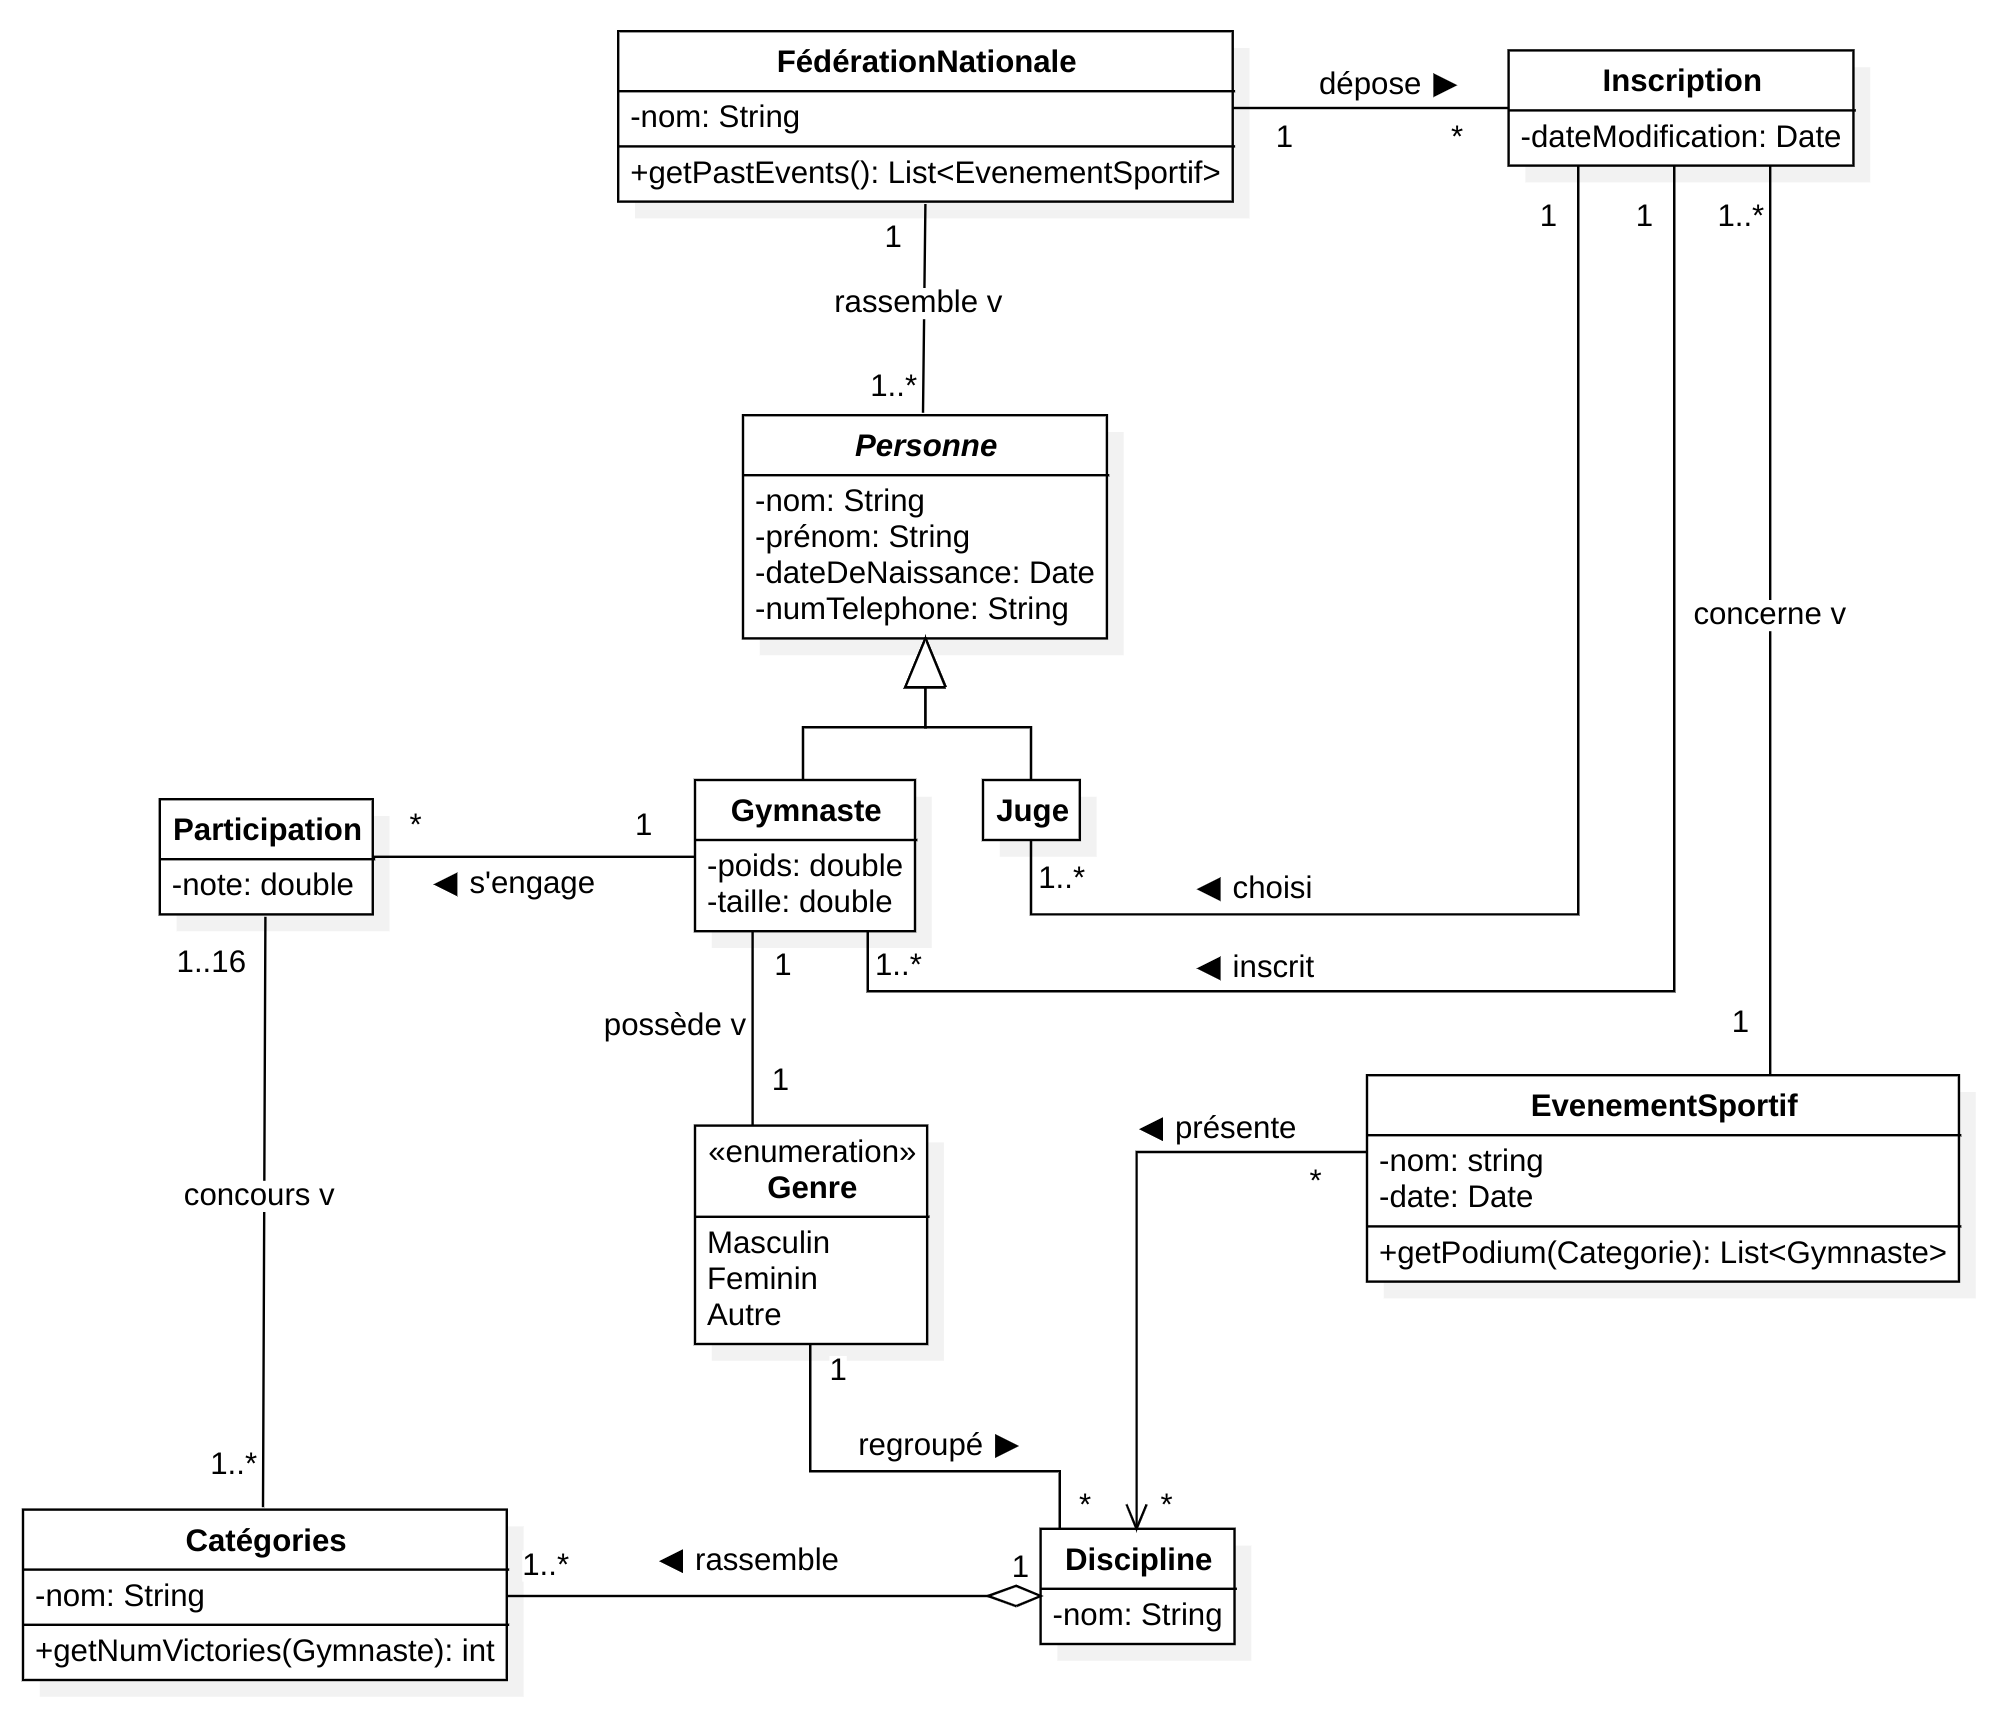
\includegraphics[width=1\textwidth]{./assets/diagram.png}
    \caption{Diagramme de classes : Fédération Internationale de Gymnastique.}
\end{figure}

\section{Contraintes d'intégrité}

\begin{itemize}
    \item Les gymnastes participant à une catégorie sont tous différents. Un même gymnaste ne peut donc pas s'inscrire deux fois dans une même catégorie.
    \item Si une discipline est présente à un évènement sportif, alors toutes ses catégories y sont présentes.
    \item Les gymnastes et juges inscrits ou choisis pour un évènement donné appartiennent à une même fédération.
    \item Un gymnaste ne peut pas participer à une catégorie s'il n'est pas inscrit à l'évènement.
    \item Une catégorie n'existe que si elle a au minimum un participant.
    \item Un gymnaste ne peut pas participer à une catégorie si elle n'est pas de son genre.
\end{itemize}
    
\section{Hypothèses de travail}

\begin{itemize}
    \item Une fédération inscrite à un évènement envoie au minimum un juge et un gymnaste.
    \item Une discipline à au minimum une catégorie.
    \item Il faut au minimum une personne pour former une fédération nationale.
    \item Les genres possibles étant connus à l'avance, ils sont définis dans une énumération.
\end{itemize}

\end{document}
